\documentclass{beamer}
\title{Circuit Partitioning and Transmission Cost Optimization in Distributed Quantum Circuits (IEEE TCAD)}
\author{Xinyu Chen, Zilu Chen, Pengcheng Zhu, Xueyun Cheng, and Zhijin Guan}
%\title{Quadratic Unconstrained Binary Optimization (QUBO)}
\date{\today}
\institute{Nantong University}
\usepackage{subcaption}
% Packages
\usepackage{tcolorbox}
\tcbuselibrary{listingsutf8}
\newtcblisting{codebox}[1][]{
	listing only,
	listing options={basicstyle=\ttfamily\footnotesize,language=Python},
	colback=gray!10,
	colframe=gray!50,
	boxrule=0.5pt,
	arc=4pt,
	outer arc=4pt,
	#1
}

\begin{document}
	
	% Title slide
	\begin{frame}
		\titlepage
	\end{frame}
	
	\begin{frame}{Motivation: Challenges in Distributed Quantum Computing}
		\begin{itemize}
			\item NISQ devices have limited qubits, preventing large-scale quantum computation.
			\item Distributed quantum computing partitions circuits across multiple QPUs.
			\item Excessive inter-QPU communication increases error rates and latency.
		\end{itemize}
	\end{frame}
	
%	\begin{frame}{Why Optimize Transmission Cost?}
%		\begin{itemize}
%			\item Transmission cost refers to overhead in quantum state transfer.
%			\item High communication frequency reduces fidelity and increases execution time.
%			\item Optimizing partitioning and scheduling can significantly reduce communication needs.
%		\end{itemize}
%	\end{frame}

	\begin{frame}{Background: state transmission}
		\begin{figure}
			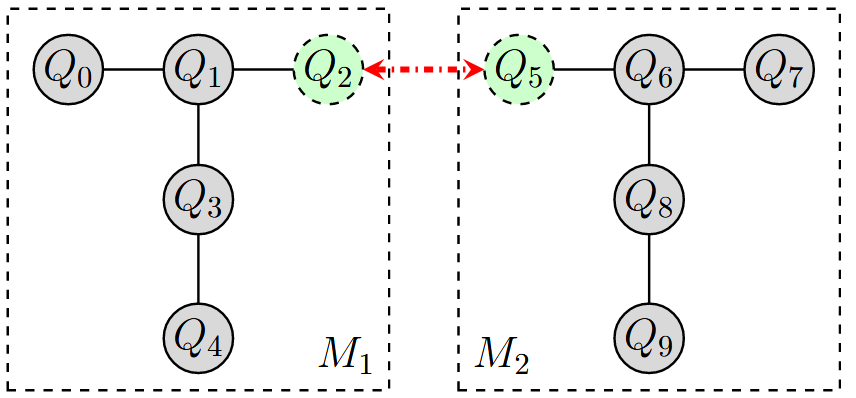
\includegraphics[width=.8\textheight]{figure/back.png}
			\caption[]{An example of a distributed quantum architecture which consists of two IBMQ quito architectures. This work focuses on direct quantum state transmission as the technology for transferring quantum states in the distributed quantum circuits.}
		\end{figure}
	\end{frame}
	
	\begin{frame}{Methodology}
		\begin{itemize}
			\item Circuit Partitioning as a Graph Cut Problem
			\item Dynamic Lookahead Transmission Optimization
		\end{itemize}
		\begin{figure}
			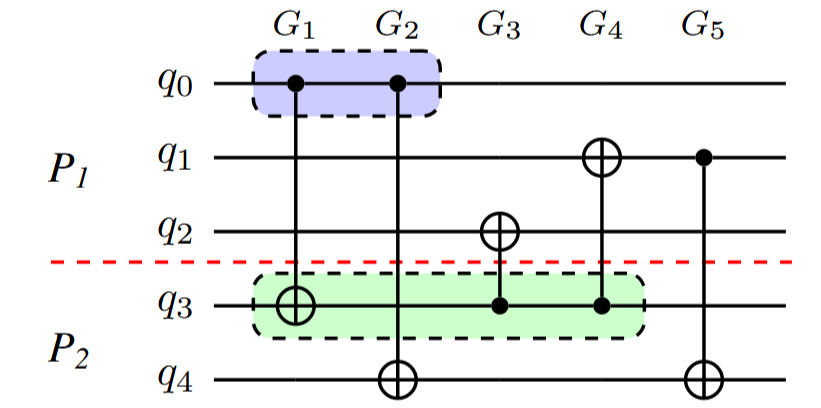
\includegraphics[width=.6\textwidth]{figure/cost.png}
			\caption{Example of the impact of transmission qubits on transmission cost. The final transmission cost of using q0 as the transmission qubit is 6, while the final transmission cost of using q3 is 4.}
		\end{figure}
	\end{frame}
	\begin{frame}{Circuit Partitioning as a Graph Cut Problem}
		\begin{itemize}
			\item Quantum circuits are represented as a qubit-weighted graph.
			\item Partitioning aims to minimize inter-QPU quantum gates.
%			\item The problem is formulated as a minimum cut optimization task.
		\end{itemize}
		\begin{figure}
			\begin{minipage}{.3\textwidth}
				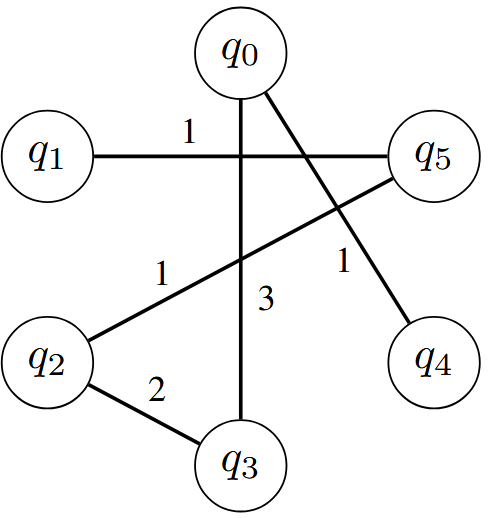
\includegraphics[width=.8\textwidth]{figure/edge.png}
%					\caption{Qubit-weighted graph with nodes as qubits, edges as quantum gates acting between qubits, and weights as the number of quantum gates.}
				
				\subcaption{}
				\label{fig:edge}
			\end{minipage}
			\begin{minipage}{.65\textwidth}
				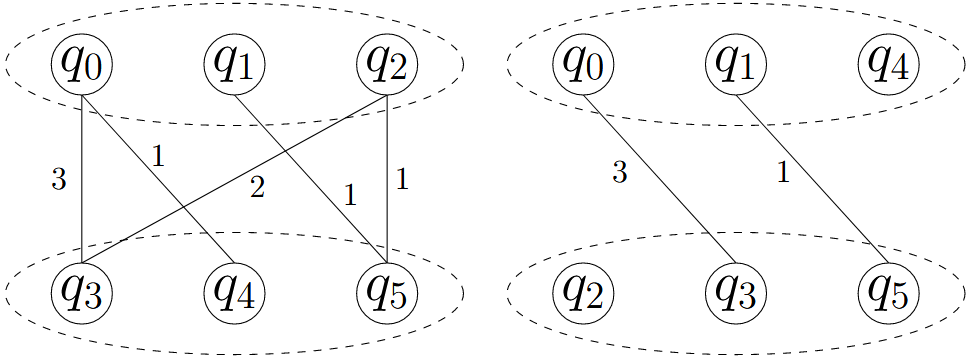
\includegraphics[width=.8\textwidth]{figure/cut.png}
%					\caption{Global gate dispersion relation graph.}
				
				\subcaption{}
				\label{fig:cut}
			\end{minipage}
			\caption[]{(\subref{fig:edge}): Qubit-weighted graph with nodes as qubits, edges as quantum gates acting between qubits, and weights as the number of quantum gates. (\subref{fig:cut}): Global gate dispersion relation graph.}
		\end{figure}
	\end{frame}
	
	% Slide: Introduction to QUBO
	\begin{frame}{Introduction to QUBO}
		\begin{itemize}
			\item \textbf{Quadratic Unconstrained Binary Optimization (QUBO)} is a mathematical model used for solving combinatorial optimization problems.
			\item It involves minimizing a quadratic function of binary variables, where each variable can be either 0 or 1.
		\end{itemize}
	\end{frame}
	
	% Slide: QUBO Objective Function
	\begin{frame}{QUBO Objective Function (from \href{https://en.wikipedia.org/wiki/Quadratic_unconstrained_binary_optimization}{wiki})}
		The general form of the QUBO objective function is:
		\[
		f(x) = x^{T} Q x = \sum_{i=1}^n \sum_{j=i}^n Q_{ij} x_i x_j
		\]
		where:
		\begin{itemize}
			\item \( x = (x_1, x_2, \ldots, x_n) \) is a vector of binary variables.
			\item \( Q \) is an upper-triangular matrix of real coefficients defining interactions between variables.
		\end{itemize}
	\end{frame}
	
	% Slide: Example of a QUBO Problem
	\begin{frame}[fragile]{Example of a QUBO Problem}
		Consider a simple QUBO problem with three binary variables:
		\[
		f(x) = Q_{11} x_1^2 + Q_{22} x_2^2 + Q_{33} x_3^2 + Q_{12} x_1 x_2 +Q_{13} x_1 x_3 + Q_{23} x_2 x_3
		\]
		Represented in matrix form:
		\[
		Q = \begin{pmatrix}
			Q_{11} & Q_{12} & Q_{13} \\
			0 & Q_{22} & Q_{23} \\
			0 & 0 & Q_{33}
		\end{pmatrix}
		\]
	\end{frame}
	\begin{frame}{Including Constraints in QUBO}
		\begin{itemize}
			\item Constraints in QUBO are introduced as penalties.
			\item Penalty functions penalize infeasible solutions.
			\item General form with constraints:
			\[
			f(x) = \sum_{i=1}^n \sum_{j=i}^n Q_{ij} x_i x_j + \sum_{k} P_k \cdot \text{penalty}_k(x)
			\]
			where:
			\begin{itemize}
				\item \(P_k\) are penalty coefficients.
				\item \(\text{penalty}_k(x)\) measures constraint violations.
			\end{itemize}
		\end{itemize}
	\end{frame}
	% Slide: Common Problems in QUBO
	\begin{frame}{Natural QUBO Formulations (from \href{https://optimization-online.org/wp-content/uploads/2019/01/7014.pdf}{A Tutorial})}
		\begin{itemize}
			\item The Number Partitioning Problem: For \( S = \{3, 1, 1, 2, 2, 1\} \), one possible partition is \( S_1 = \{1, 1, 1, 2\} \) and \( S_2 = \{2, 3\} \), both summing to 5.
			
			\item The Max Cut Problem: In a triangle graph with vertices \( \{A, B, C\} \) and edges \( \{(A, B), (B, C), (C, A)\} \), one maximum cut is \( S = \{A\} \) and \( \bar{S} = \{B, C\} \), resulting in two edges crossing the cut.
		\end{itemize}
		\begin{itemize}
			\item Various algorithms can solve QUBO problems, including \textbf{Quantum annealing methods using quantum computers}. (Ref. [\href{https://arxiv.org/pdf/1811.11538}{1811.11538},\href{https://www.nature.com/articles/s41598-019-53585-5}{s41598-019-53585-5}])
		\end{itemize}
	\end{frame}
	
	\begin{frame}{Comparison with Existing Methods}
		\begin{figure}
			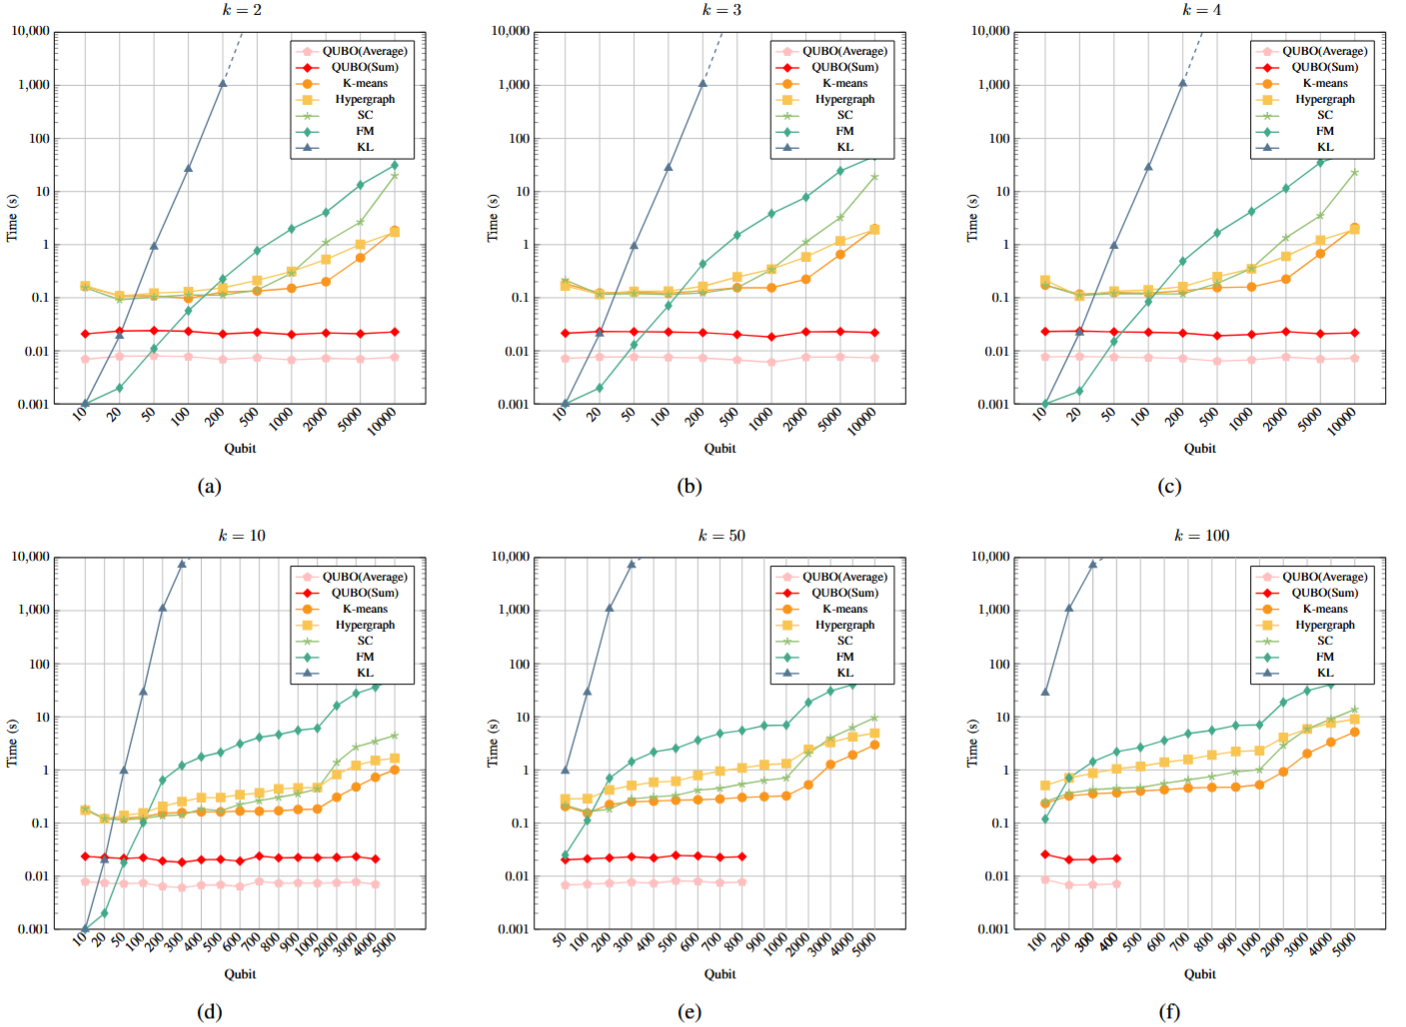
\includegraphics[width=0.8\textwidth]{figure/time.png}  % Replace with actual data visualization
			\caption{Comparison of runtime performance between the QUBO model-based and other circuit partitioning methods under different numbers of qubits and partition counts k.}
		\end{figure}
	\end{frame}
	
	\begin{frame}{Dynamic Lookahead Transmission Optimization}
		\begin{itemize}
%			\item Transmission qubit selection is crucial for reducing communication.
			\item Looks ahead dynamically to evaluate impact of transmission choices. Prioritizes merging quantum gate executions to minimize state transfers.
		\end{itemize}
		\begin{figure}
			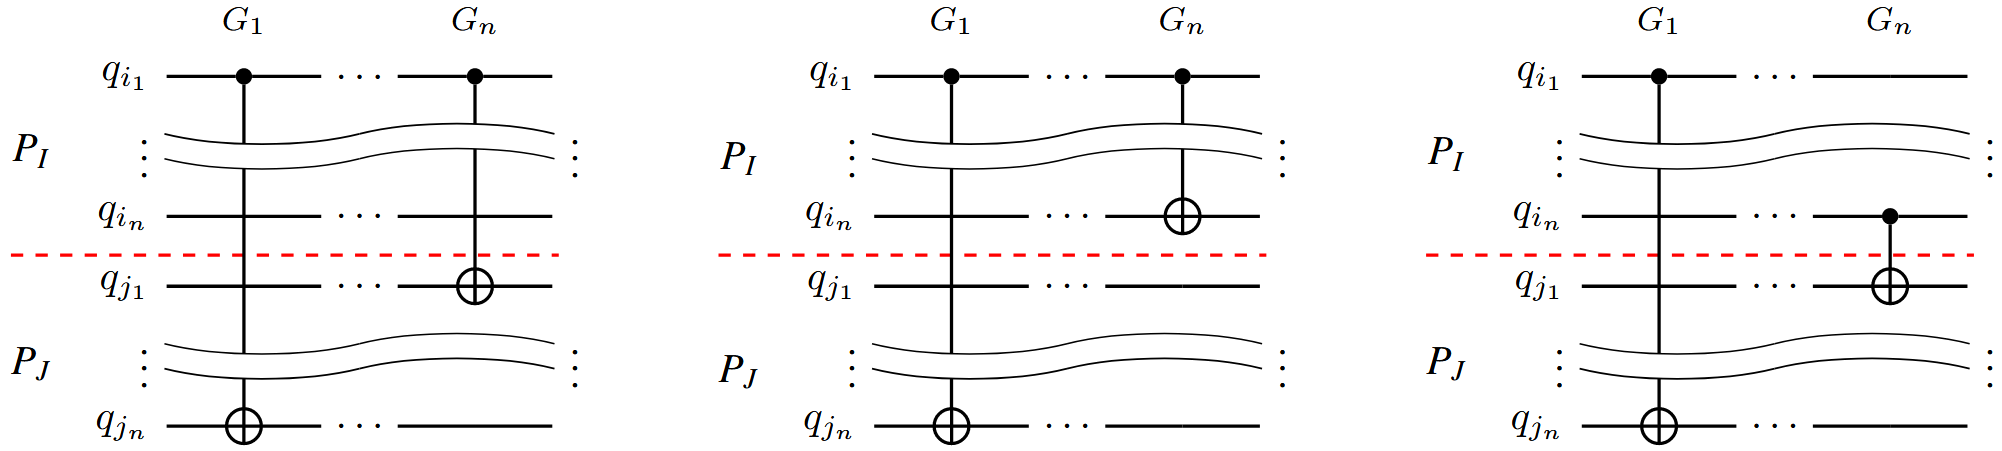
\includegraphics[width=.9\textwidth]{figure/transfer.png}
			\caption{The different impacts of transferring qubit $q_{i1}$ on subsequent gates.}
		\end{figure}
	\end{frame}
	
	\section{Results}
	\begin{frame}{Performance Gains}

		\begin{itemize}
			%		RevLib used 
			\item Achieving an average optimization rate of 18.12\% and a peak rate of 73.85\% in transmission cost compare with meta-heuristic methods.
			\item Achieving an average optimization rate of 32.27\% and a peak rate of 55.56\% with greedy strategies.
		\end{itemize}
		\begin{figure}
			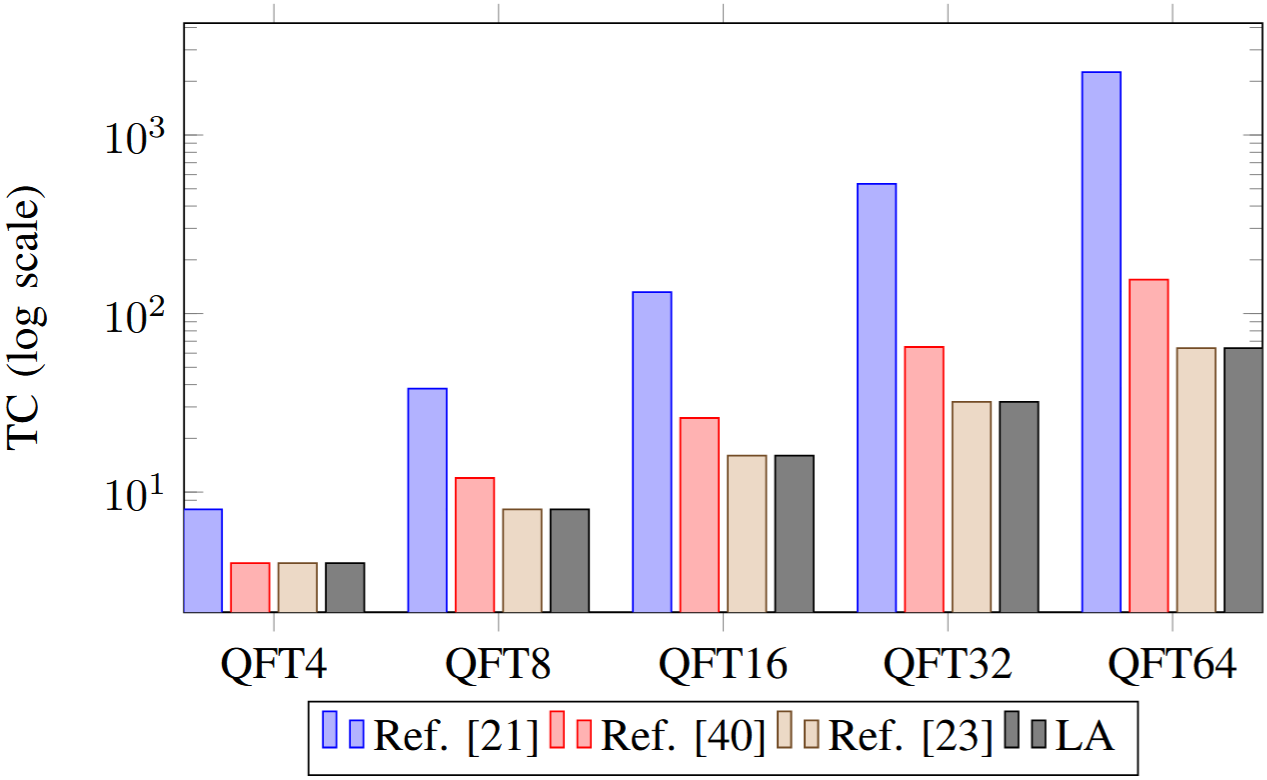
\includegraphics[width=.6\textwidth]{figure/TC.png}
			\caption[]{Bar chart comparing the transmission cost results in QFT circuits.}
		\end{figure}
	\end{frame}
	
	
	\begin{frame}{Conclusion}
		\begin{itemize}
			\item Proposed QUBO-based partitioning reduces inter-QPU gates.
			\item Dynamic lookahead scheduling significantly lowers transmission cost.
			\item Approach enables more efficient execution of distributed quantum algorithms.
		\end{itemize}
	\end{frame}
	
%	\begin{frame}{Future Directions}
%		\begin{itemize}
%			\item Extend QUBO approach for more than 100 partitions.
%			\item Incorporate error rates and latency in transmission models.
%			\item Test method in real quantum hardware environments.
%		\end{itemize}
%	\end{frame}
	
	
%	 Slide: Solving the QUBO Problem
%	\begin{frame}{Solving the QUBO Problem}
%		\begin{itemize}
%			\item Various algorithms can solve QUBO problems, including:
%			\begin{itemize}
%				\item Exact algorithms like Branch and Bound.
%				\item Approximate algorithms like Simulated Annealing.
%				\item 
%%				\href{https://arxiv.org/abs/1705.09844}{Quadratic Unconstrained Binary Optimization Problem Preprocessing: Theory and Empirical Analysis.}
%			\end{itemize}
%		\end{itemize}
%	\end{frame}
	
	% Slide: Constraints in QUBO
	
	
%	% Example of constraint
%	\begin{frame}{Constraint Example}
%		Consider the constraint:
%		\[ \sum_{i=1}^n x_i = 2 \]
%		This can be incorporated using a quadratic penalty:
%		\[
%		\text{penalty}(x) = \left(\sum_{i=1}^n x_i - 2\right)^2
%		\]
%		Expanded form:
%		\[
%		\left(\sum_{i=1}^n x_i - 2\right)^2 = \sum_{i=1}^n \sum_{j=1}^n x_i x_j - 4\sum_{i=1}^n x_i + 4
%		\]
%		The penalty is zero when exactly two variables equal one.
%	\end{frame}
%		
%		% Slide with constraints in code
%	\begin{frame}[fragile]{Incorporating Constraints in Code}
%		Example Python snippet illustrating constraints:
%		\begin{codebox}
%Q = [[1, -1, 2],
%[0, 1, -3],
%[0, 0, 1]]
%
%# Constraint: exactly two variables equal 1
%penalty = lambda x: (sum(x) - 2)**2
%
%# Total objective
%objective = lambda x: x @ Q @ x + 10 * penalty(x)
%
%# Hypothetical solver usage
%# solution = solve_qubo(objective)
%		\end{codebox}
%	\end{frame}
	% Slide: Applications of QUBO
%	\begin{frame}{Applications of QUBO}
%		QUBO models are utilized in various fields, including:
%		\begin{itemize}
%			\item \textbf{Machine Learning}: Feature selection, clustering, and support vector machines.
%			\item \textbf{Operations Research}: Problems like the traveling salesperson, vehicle routing, and scheduling.
%			\item \textbf{Quantum Computing}: Serving as the foundational problem format for quantum annealers and certain quantum algorithms.
%		\end{itemize}
%	\end{frame}
	
\end{document}
